\documentclass[a4]{beamer}
\usepackage{amssymb}
\usepackage{graphicx}
\usepackage{subfigure}
\usepackage{newlfont}
\usepackage{amsmath,amsthm,amsfonts}
%\usepackage{beamerthemesplit}
\usepackage{pgf,pgfarrows,pgfnodes,pgfautomata,pgfheaps,pgfshade}
\usepackage{mathptmx} % Font Family
\usepackage{helvet} % Font Family
\usepackage{color}
\mode<presentation> {
\usetheme{Default} % was Frankfurt
\useinnertheme{rounded}
\useoutertheme{infolines}
\usefonttheme{serif}
%\usecolortheme{wolverine}
% \usecolortheme{rose}
\usefonttheme{structurebold}
}
\setbeamercovered{dynamic}
\title[MA4413]{Statistics for Computing \\ {\normalsize MA4413 Lecture 11A}}
\author[Kevin O'Brien]{Kevin O'Brien \\ {\scriptsize kevin.obrien@ul.ie}}
\date{Autumn 2013}
\institute[Maths \& Stats]{Dept. of Mathematics \& Statistics, \\ University \textit{of} Limerick}
\renewcommand{\arraystretch}{1.5}
%------------------------------------------------------------------------%

\begin{document}
\begin{frame}
\titlepage
\end{frame}

\begin{frame}
\frametitle{Discrete memoryless channel (from last lecture)}
\begin{itemize}
\item For a DMC with ``m" inputs and ``n" outputs, the input X consists of input symbols $x_1, x_2, \ldots x_m$.
\item The probabilities of these source symbols $P(x_i)$ are assumed to be known.
\item The output Y consists of output symbols $\{y_1,y_2,\ldots, y_n \}$
\item Each possible input-to-output path is indicated along with a conditional probability $P(y_j|x_i)$, where $P(y_j|x_i)$  is the conditional probability of
obtaining output $y_j$ given that the input is $x_i$. \item $P(y_j|x_i)$ is called a \textbf{\emph{channel transition probability}}.
\end{itemize}
\end{frame}
%\end{document}
%--------------------------------------------------------%
%--------------------------------------------------------%
\begin{frame}
\frametitle{Discrete memoryless channel}
\vspace{-1cm}
\begin{itemize}
\item On the next slide, we present a binary DMC, with the channel transition probabilities indicated.
\item $P(y_1|x_1)$ = 0.9  and $P(y_2|x_1)$ = 0.1
\item $P(y_1|x_2)$ = 0.2  and $P(y_2|x_2)$ = 0.8
\end{itemize}
\end{frame}

\frame{
\frametitle{Discrete Memoryless Channels}

\begin{center}
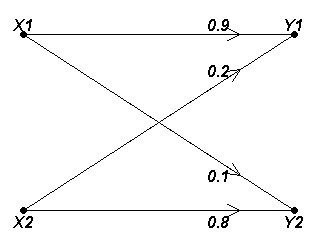
\includegraphics[scale=0.54]{10Bnet2}
\end{center}
}
%- Data Compression ( www.datacompression.com )

\begin{frame}
\frametitle{Channel Matrix}

A channel is completely specified by the complete set of transition probabilities. Accordingly, a
channel is specified by the matrix of transition probabilities $[P(Y|X)]$, given by

\[  [P(Y|X)]  = \left[ \begin{array}{cccc}
P(y_1|x_1) & P(y_2|x_1) & \ldots & P(y_n|x_1) \\
P(y_1|x_2) & P(y_2|x_2) & \ldots & P(y_n|x_2) \\
\ldots & \ldots & \ldots & \ldots \\
P(y_1|x_m) & P(y_2|x_m) & \ldots & P(y_n|x_n) \\
\end{array} \right] \]


The matrix $[P(Y|X)]$ is called the \textbf{\emph{channel matrix}}.
%ZP(yylx;) : l lor all 1 (10.12)
 \end{frame}

\begin{frame}
\frametitle{Channel Matrix}
\begin{itemize}
\item Since each input to the channel results in some
output, each row of the channel matrix must sum to unity (i.e. all rows must add up to 1. This condition is not necessary for columns).
\item For the binary DMC presented previously, the channel matrix is
\[  [P(Y|X)]  = \left[ \begin{array}{cc}
0.9 & 0.1  \\
0.2 & 0.8 \\
\end{array} \right] \]
\item (Remark: This is not the same as a binary symmetric channel (relevant to later material)
\end{itemize}
\end{frame}


\begin{frame}
\frametitle{Channel Matrix}
\begin{itemize}
\item The input probabilities $P(X)$ are represented by the row matrix
\[  [P(X)]  = \left[ \begin{array}{cccc}
P(x_1) & P(x_2) & \ldots & P(x_m) \\
\end{array} \right] \]
\item The output probabilities $P(Y)$ are represented by the row matrix
\[  [P(Y)]  = \left[ \begin{array}{cccc}
P(y_1) & P(y_2) & \ldots & P(y_n) \\
\end{array} \right] \]
\item We can compute $[P(Y)] $ by the following formula: $[P(Y)]  = [P(X)]\times [P(Y|X)]$
\item (Note: Be mindful of the dimensions of each matrix).
\end{itemize}
\end{frame}

\begin{frame}
\frametitle{Channel Matrix}
\begin{itemize}
\item Suppose for our Binary DMC that the input probabilities were given by $[P(X)] = [ 0.5\mbox{   }0.5]$.
\item Compute $[P(Y)]$, given the channel matrix given in previous slides.
\[  [P(Y)]  =  \left[ \begin{array}{cc}
0.5 & 0.5 \\
\end{array} \right] \times \left[ \begin{array}{cc}
0.9 & 0.1  \\
0.2 & 0.8 \\
\end{array} \right] \]

\item Solving
\[  [P(Y)]  =  \left[ \begin{array}{cc}
(0.5 \times 0.9)+(0.5 \times 0.2) & (0.5 \times 0.1)+(0.5 \times 0.8) \\
\end{array} \right]  \]

\item Simplifying \[  [P(Y)]  =  \left[ \begin{array}{cc}
0.55 & 0.45 \\
\end{array} \right]  \]
\end{itemize}
\end{frame}


\begin{frame}
\frametitle{Channel Matrix}
\begin{itemize}
\item Let $[P(X)]$ is presented as a diagonal matrix , i.e.

\[  [P(X)]_d  = \left[ \begin{array}{cccc}
P(x_1) &0 & \ldots & 0 \\
0 & P(x_2)& \ldots & 0 \\
\ldots & \ldots & \ldots & \ldots \\
0& 0 & \ldots & P(x_m) \\
\end{array} \right] \]
\item The \emph{\textbf{ joint probability matrix}} $[P(X,Y)]$can be computed as
$[P(X,Y)]  = [P(X)]_d\times [P(Y|X)]$
\end{itemize}
\end{frame}

\begin{frame}
\frametitle{Channel Matrix}
\begin{itemize}
\item For the Binary DMC described in the previous example, compute the joint probability matrix.
\item Diagonalize the input probabilities for $X$.
\[  [P(X)]_d  = \left[ \begin{array}{cc}
0.5 & 0.0  \\
0.0 & 0.5\\
\end{array} \right] \]

\item Simplifying
\[  [P(X,Y)]  =  \left[ \begin{array}{cc}
(0.5 \times 0.9)+(0 \times 0.2) & (0.5 \times 0.1)+(0 \times 0.8) \\
(0 \times 0.9)+(0.5 \times 0.2) & (0 \times 0.1)+(0.5 \times 0.8) \\
\end{array} \right]  \]


\item Solving
\[  [P(X,Y)]  =  \left[ \begin{array}{cc}
0.45 & 0.05 \\
0.1  & 0.4 \\
\end{array} \right]  \]
\end{itemize}
\end{frame}
%---------------------------------------------------------------------------------------------------------------------------------------------------%
\begin{frame}
\frametitle{Types of Channel}
\textbf{ 1. Lossless Channel:}\\
A channel described by a channel matrix with only one non-zero element in each column is called a lossless channel.


\[  [P(Y|X)]  =  \left[ \begin{array}{ccccc}
3/4 & 1/4 &0 & 0&0\\
0  & 0 &1/3 & 2/3& 0\\
0  & 0& 0&0 &1 \\
\end{array} \right]  \]
%(Drawn in overhead):\\ \bigskip

It can be shown that in the lossless channel, no source information is lost in transmission.
\end{frame}
%---------------------------------------------------------------------------------------------------------------------------------------------------%
\begin{frame}
\frametitle{Types of Channel}
\textbf{ 1. Lossless Channel:}\\

\begin{figure}
\centering
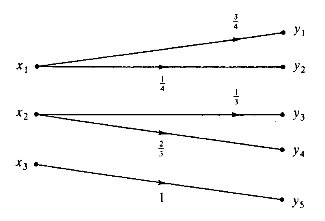
\includegraphics[width=0.7\linewidth]{./11Blossless}
\caption{}
\label{fig:11Blossless}
\end{figure}


\end{frame}

%---------------------------------------------------------------------------------------------------------------------------------------------------%
\begin{frame}
\frametitle{Types of Channel}
\textbf{2. Deterministic Channel:}\\
A channel described by a channel matrix with only one non-zero element in each row is called a deterministic channel.

\[  [P(Y|X)]  =  \left[ \begin{array}{ccc}
1   & 0 &0 \\
1  & 0 &0\\
0  & 1 &0\\
0  & 1& 0 \\
0  & 0& 1 \\
\end{array} \right]  \]
%(Drawn in overhead):\\ \bigskip
Note that since each row has only one non-zero element, this element must be 1. When a given source symbol is sent in a deterministic channel, it is clear which output symbol would be received.
\end{frame}

%---------------------------------------------------------------------------------------------------------------------------------------------------%
\begin{frame}
\frametitle{Types of Channel}
\textbf{2. Deterministic Channel:}\\
\begin{figure}
\centering
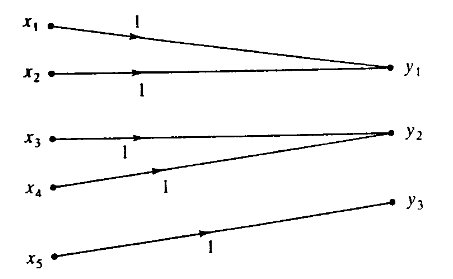
\includegraphics[width=0.7\linewidth]{./11Bdeterministic}
\caption{}
\label{fig:11Bdeterministic}
\end{figure}

\end{frame}

%---------------------------------------------------------------------------------------------------------------------------------------------------%
\begin{frame}
\frametitle{Types of Channel}
\textbf{3. Noiseless Channel:}\\
A channel is said to be \emph{\textbf{noiseless}} if it is both lossless and deterministic.
The channel matrix is the identity matrix: only one element in each row and each column, and each element is necessarily 1.
\[  [P(Y|X)]  = \left[ \begin{array}{cccc}
1 &0 & \ldots & 0 \\
0 & 1& \ldots & 0 \\
\ldots & \ldots & \ldots & \ldots \\
0& 0 & \ldots & 1 \\
\end{array} \right] \]
%(Drawn in overhead):\\ \bigskip
Note that the input and output alphabets have the same size , i.e. $m=n$.
\end{frame}
\begin{frame}
\frametitle{Types of Channel}
\textbf{3. Noiseless Channel:}\\
\begin{figure}
\centering
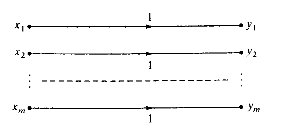
\includegraphics[width=0.7\linewidth]{./11BNoiseless}
\caption{}
\label{fig:11BNoiseless}
\end{figure}

\end{frame}
%----------------------------------------------------------------------------------------------------------------------------------------------------%
\begin{frame}
\frametitle{Types of Channel}
\textbf{4. Binary Symmetric Channel:}\\
The binary symmetric channel is defined by the following channel diagram (next slide) and the channel matrix is given by

\[  [P(Y|X)]  = \left[ \begin{array}{cc}
1-p & p  \\
p & 1-p\\
\end{array} \right] \]
The channel has two inputs and two outputs $(x_1=0,x_2=1)$ and two outputs $(x_1=0,x_2=1)$. The channel is symmetric because the probability of receiving a 1 if a 0 is sent is the same as the probability of receiving a 0 if a 1 was sent. This common probability is denoted $p$.
\end{frame}

\frame{
\frametitle{Binary Symmetric Channels}

\begin{center}
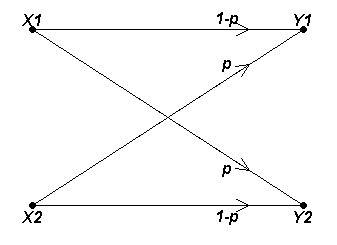
\includegraphics[scale=0.54]{11aBSC}
\end{center}
}


\begin{frame}
\frametitle{Mutual Information}
Mutual information is one of many quantities that measures how much one random variables gives about another. It is a dimensionless quantity. Mutual Informaiton can be thought of as the reduction in uncertainty about one random variable given knowledge of another. 
\begin{itemize}\item High mutual information indicates a large reduction in uncertainty, \item low mutual information indicates a small reduction, \item  zero mutual information between two random variables means the variables are independent.
\end{itemize}
Efficient communication systems have high mutual information.
\end{frame}
%---------------------------------------------------------------------------------------------------------------------------------------%
\begin{frame}
\frametitle{Mutual Information}
\vspace{-1cm}
\textbf{Joint Entropies:}\\
Using the input probabilities $P(x_i)$, output probabilities $P(y_i)$, transition probabilities $P(y_i|x_i)$,
and joint probabilities $P(x_i,y_j)$, we can define the following various entropy functions for a channel
with m inputs and n outputs:

\begin{itemize}
\item $H(X) = - \sum ^{m}_{i=1} P(x_i) \mbox{log}_2 P(x_i)$%; P(x;) (10.21)
\item $H(Y) = - \sum ^{n}_{j=1} P(y_j) \mbox{log}_2 P(y_j)$
\item $H(X, Y)= - \sum ^{n}_{j=1}\sum ^{m}_{i=1} P(x_i,y_j) \mbox{log}_2 P(x_i,y_j)$
\end{itemize}
\end{frame}

%---------------------------------------------------------------------------------------------------------------------------------------%
\begin{frame}
\frametitle{Mutual Information: Joint Entropy}
\vspace{-1cm}
These entropies can be interpreted as follows:\begin{itemize}\item $ H(X)$ is the average uncertainty of the channel input,
and $H(Y)$ is the average uncertainty of the channel output.\item  The joint entropy $H(X,Y)$ is the average uncertainty of the communication channel as a
whole.\end{itemize}
\end{frame}
%---------------------------------------------------------------------------------------------------------------------------------------%
\begin{frame}
\frametitle{Mutual Information: Conditional Entropy}
\begin{itemize}
\item The conditional entropy $H(X|Y)$ is a
measure of the average uncertainty remaining about the channel input after the channel output has
been observed. \item This is sometimes called the equivocation of X with respect to Y.  \item The
conditional entropy $H(Y|X)$ is the average uncertainty of the channel output given that X was
transmitted.
\end{itemize}
\begin{itemize}
\item $H(X|Y)= - \sum ^{n}_{j=1}\sum ^{m}_{i=1} P(x_i,y_j) \mbox{log}_2 P(x_i|y_j)$
\item $H(Y|X)= - \sum ^{n}_{j=1}\sum ^{m}_{i=1} P(x_i,y_j) \mbox{log}_2 P(y_j|x_i)$
\end{itemize}
\end{frame}
%-----------------------------------------------------------------------------------------------%
\begin{frame}
\frametitle{Mutual Information : Useful Identities}
Two useful relationships among the types of entropies are
\begin{itemize}
\item $H(X,Y)=H(X|Y)+H(Y) $
\item $H(X,Y)=H(Y|X)+H(X) $
\end{itemize}
(Remark : compare to identities in probability theory)
\end{frame}
%-----------------------------------------------------------------------------------------------%
\begin{frame}
\frametitle{Mutual Information : Useful Identities}
\begin{figure}
\centering
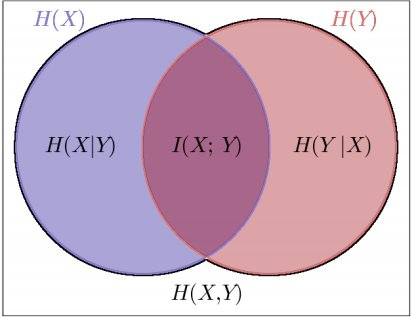
\includegraphics[width=0.7\linewidth]{./11BMutualInfo}
\caption{}
\label{fig:11BMutualInfo}
\end{figure}


\end{frame}



\begin{frame}

\frametitle{Mutual Information}
The mutual information $I(X; Y)$ of a channel is defined by
\[ I(X; Y) = H(X) -  H(X|Y) \mbox{    (b/symbol) } \]

Alternatively we can define it as either
\[ I(X; Y) = H(Y) -  H(Y|X) \mbox{     (b/symbol) } \]
 or as
\[ I(X; Y) = H(Y)+ H(Y)  - H(X,Y) \mbox{    (b/symbol) } \]
Remark: The
mutual information is the reduction of
entropy of X when Y
is
known.
\end{frame}

%----------------------------------------------------------------------------------%
\frame{
\frametitle{Entropy: some remarks}
\begin{itemize}
\item recall: Entropy is the uncertainty of a single random variable. \item We can define \textbf{\emph{conditional entropy }}$H(X|Y)$, which is the entropy of a random variable
conditional on the knowledge of another random variable. \item The reduction in uncertainty due to another random variable is called the \textbf{\emph{mutual information}}.
\end{itemize}
}
%----------------------------------------------------------------------------------%
\begin{frame}
\frametitle{Entropies: Example}
\begin{itemize}
\item The input source to a noisy communication channel is a random variable X over the
four symbols $\{a, b, c, d\}$. \item  The output from this channel is a random variable Y over these same
four symbols.
\end{itemize}

\end{frame}
%----------------------------------------------------------------Part 2 %
\begin{frame}
\frametitle{Entropies: Example}
The joint distribution of these two random variables is as follows:\\ \bigskip
\begin{center}
\begin{tabular}{|c|c|c|c|c|}
\hline
&x=a& x=b & x=c & x=d \\ \hline
y=a &1/8 &1/16 &1/16 &1/4 \\ \hline
y=b &1/16 & 1/8& 1/16& 0 \\ \hline
y=c & 1/32&1/32 & 1/16 & 0\\ \hline
y=d & 1/32& 1/32& 1/16 & 0\\ \hline
\end{tabular}
\end{center}
\end{frame}
%----------------------------------------------------------------Part 2 %
\begin{frame}
\frametitle{Entropies: Example}
\begin{itemize}
\item Write down the marginal distribution for $X$ and compute the marginal entropy $H(X)$.
\item Write down the marginal distribution for $Y$ and compute the marginal entropy $H(Y )$.
\item (next class) What is the joint entropy $H(X, Y ) $ of the two random variables?
\item (next class) What is the conditional entropy $H(Y|X)$?
\item (next class) What is the conditional entropy $H(X|Y)$?
\item (next class) What is the mutual information $I(X;Y)$ between the two random variables?
\end{itemize}
\end{frame}
%----------------------------------------------------------------------------------%
%----------------------------------------------------------------Part 2 %
\begin{frame}
\frametitle{Entropies: Example}
The marginal distribution of these two random variables is as follows:\\ \bigskip
\begin{center}
\begin{tabular}{|c|c|c|c|c||c|}
\hline
&x=a& x=b & x=c & x=d &\alert{P(Y)}\\ \hline
y=a &1/8 &1/16 &1/16 &1/4 & \alert{0.50}\\ \hline
y=b &1/16 & 1/8& 1/16& 0 & \alert{0.25}\\ \hline
y=c & 1/32&1/32 & 1/16 & 0& \alert{0.125}\\ \hline
y=d & 1/32& 1/32& 1/16 & 0& \alert{0.125}\\ \hline \hline
\alert{P(X)} & \alert{0.25}& \alert{0.25}& \alert{0.25} & \alert{0.25}&\\ \hline
\end{tabular}
\end{center}
\end{frame}


\begin{frame}
\frametitle{Entropies: Example}
\begin{itemize}

\item H(X) , the entropy of X, is computed as\\
 \[H(X) = -\sum P(x_i) \mbox{log}_2P(x_i)\] \item $H(X) =  (-0.25 \times -2) + (-0.25 \times -2) +(-0.25 \times -2) +(-0.25 \times -2)$\item $ H(X) = 2 \mbox{b}$ \bigskip

\item H(X) , the entropy of Y, is computed as\\
 \[H(Y) = -\sum P(y_j) \mbox{log}_2P(y_j)\] \item $H(Y) =  (-0.5 \times -1) +(-0.25 \times -2)  + (-0.125 \times -3)  +(-0.125 \times -3)$\item $ H(Y) = 1.75 \mbox{b}$


\end{itemize}
\end{frame}


\end{document}
%---------------------------------------------------------------------------------------------------------------------------------------%

\begin{frame}
\frametitle{Channel Capacity}

\textbf{A. Channel Capacity per Symbol C:}\\
The channel capacity per symbol of a DMC is defined as
\[
C. = \mbox{max }I(X; Y) \mbox{ b/symbol }
\]
where the maximization is over all possible input probability distributions {P(x,)} on X. Note that the
channel capacity CA is a function of only the channel transition probabilities that define the channel.
\textbf{B. Channel Capacity per Second C:}\\
If r symbols are being transmitted per second, then the maximum rate of transmission of
information per second is rC>.. This is the channel capacity per second and is denoted by C (bls):
C : rC, b/s
\end{frame}

%------------------------------------------------------------------------%



%---------------------------------------------------------------------------------Page 251 C-%
\begin{frame}
\frametitle{Capacities of special channels}
\textbf{\emph{Lossless Channel}}:  $H(X|Y) = 0$ Therefore $I(X;Y) = H(X)$.
The mutual information (information transfer) is equal to the input (source) entropy), and no source information is lost in transmission, Consequently, the channel capacity per symbol is
\[ C_s = \mbox{ max }_{P(x_i)} H(X) = \mbox{log}_2m \]
where $m$ is the number of symbols in $X$.

\end{frame}
\end{document}
%---------------------------------------------------------------------------------Page 251 D-%
\begin{frame}
\frametitle{Capacities of special channels}
\begin{itemize}
\item \textbf{\emph{Deterministic Channel}}:  $H(Y|X) = 0$ Therefore $I(X;Y) = H(Y)$.
The mutual information (information transfer) is equal to the output entropy). The channel capacity per symbol is
\[ C_s = \mbox{ max }_{P(x_i)} H(Y) = \mbox{log}_2n \]
where $n$ is the number of symbols in $Y$.
\end{itemize}
\end{frame}
%---------------------------------------------------------------------------------Page 252 A -%
\begin{frame}
\frametitle{Capacities of special channels}
\begin{itemize}
\item \textbf{\emph{Noiseless Channel}}:  Since a noiseless channel is both lossless and deterministic , we can say that $I(X;Y) = H(X) = H(Y)$.
The mutual information (information transfer) is equal to the output entropy). The channel capacity per symbol is
\[ C_s = \mbox{log}_2m = \mbox{log}_2n \]
\end{itemize}
\end{frame}


% - Lossless data compression.
% - Huffman Coding
% - Inverse Mapping

\end{document}

%-----------------------------------------------------------------Part 3 Data Compression %

\frame{
\frametitle{Data compression(1)}
Data compression is the science (and art) of representing information in a compact form. Having been the domain of a relatively small group of engineers and scientists, it is now ubiquitous. \\ \bigskip It has been one of the critical enabling technologies for the on-going digital multimedia revolution for decades. Without compression techniques, none of the ever-growing Internet, digital TV, mobile communication or increasing video communication would have been practical developments. \\ \bigskip
}
%-----------------------------------------------------------------------------------------------%
\frame{
\frametitle{Data compression(1)}

Data compression is an active research area in computer science. By "compressing data", we actually mean deriving techniques or, more specifically, designing efficient algorithms to:

\begin{itemize}
\item represent data in a less redundant fashion
\item remove the redundancy in data
\item implement coding, including both encoding and decoding.
\end{itemize}

}


\end{document}


%----------------------------------------------------------------Part 4 Huffman Coding-%

\frame{
\frametitle{Huffman encoding algorithm}
Huffman coding is an entropy encoding algorithm used for lossless data compression.\\
\bigskip
A frequency based coding scheme (algorithm) that follows Huffman's idea is called Huffman coding. Huffman coding is a simple algorithm that generates a set of variable-size codewords of the minimum average length. The algorithm for Huffman encoding involves the following steps:
}
%--------------------------------------------------------------Part 4 Huffman Coding-%

\frame{
\begin{itemize}
\item[1.] Frequency Table: Constructing a frequency table sorted in descending order.

\item[2.] Building a binary tree:
    Carrying out iterations until completion of a complete binary tree:
    \begin{itemize}
    \item[(a)] Merge the last two items (which have the minimum frequencies) of    the frequency table to form a new combined item with a sum
    frequency of the two.
    \item[(b)] Insert the combined item and update the frequency table.
    \end{itemize}

\item[3.] Deriving Huffman tree:
Starting at the root, trace down to every leaf; mark �0� for a left branch and �1� for a right branch.

\item[4.] Generating Huffman code:
Collecting the 0s and 1s for each path from the root to a leaf and assigning a 0-1 codeword for each symbol.

\end{itemize}
}
%--------------------------------------------------------------------------Part 4 Huffman Coding-%

\frame{

Huffman coding is a method of lossless data compression, and a form of entropy encoding. The basic idea is to map an alphabet to a representation for that alphabet, composed of strings of variable size, so that symbols that have a higher probability of occurring have a smaller representation than those that occur less often.

}
%-------------------------------------------------------------------------------Part 4 Huffman Coding-%

\frame{
The key to Huffman coding is Huffman's algorithm, which constructs an extended binary tree of minimum weighted path length from a list of weights. For this problem, our list of weights consists of the probabilities of symbol occurrence. From this tree (which we will call a Huffman tree for convenience), the mapping to our variable-sized representations can be defined.
}
%-----------------------------------------------------------------------Part 4 Huffman Coding-%
\frame{
The mapping is obtained by the path from the root of the Huffman tree to the leaf associated with a symbol's weight. The method can be arbitrary, but typically a value of 0 is associated with an edge to any left child and a value of 1 with an edge to any right child (or vice-versa). By concatenating the labels associated with the edges that make up the path from the root to a leaf, we get a binary string. Thus the mapping is defined.
}
%-------------------------------------------------------------------------------------------%
\frame{
\frametitle{Inverse Mapping}
\begin{itemize}
\item In order to recover the symbols that make up a string from its representation after encoding, an inverse mapping must be possible. It is important that this mapping is unambiguous. \item We can show that all possible strings formed by concatenating any number of path labels in a Huffman tree are indeed unambiguous, due to the fact that it is a complete binary tree. \item That is, given a string composed of Huffman codes, there is exactly one possible way to decompose it into the individual codes.
\end{itemize}
}

\frame{
\frametitle{Data compression(2)}
The key approaches of data compression can be summarized as modelling + coding.
Modelling is a process of constructing a knowledge system for
performing compression. Coding includes the design of the code and product of the compact data form.

}

% - Entropy
% - Information
% - Mutual Information



%-------------------------------------------------------------------------------------------------------------------------------------------------------------------------------------------%


% page 247






%r. - · yi
%XI: X Ptytnt ykzyr
%rn,. · yn



\begin{frame}
\frametitle{Code efficiency and Code redundancy}
% Pg 253/254
The parameter $L$ represents the average number of bits per source symbol used in the source coding process.
The code efficiency is defined as \[\nu = {L_{min} \over L} \]where $L_{min}$ is the minimum possiblve value of $L$. When $\nu$ approaches unity, the codes is said to be efficient.
The code redundancy $\gamma$ is defined as $\gamma = 1- \nu$.
\end{frame}


%---------------------------------------------------------------------------------------------------------------------------------------%
\begin{frame}
%page 254
\frametitle{Source Coding Theorem}
The source coding theorem states that for zi DMS X with entropy $H(X)$, the average code word length $L$ per symbol is bounded as
L 2 H(X) (10.52)

and further, L can bc made as close to H(X) as dcsircd for some suitably chosen code.
Thus, with$ L_{min} \geq H(X)$.

The code efficiency can be rewritten as
\[\nu = {H(X) \over L} \]
\end{frame}

%---------------------------------------------------------------------------------------------------------------------------------------%
\begin{frame}
\frametitle{ Classification of Codes}
Classification of codes is best illustrated by an example. Consider Table 10-1 where a source of
size 4 has been encoded in binary codes with symbol 0 and 1.\\ \bigskip
% Table 10-I Binary Codes
\begin{tabular}{c c c c c c c}
X& Code l& Code 2& Code 3 &Code 4& Code 5& Code 6\\
a& 01& 01 &1 &10 &01 &01\\
b& 01& 01 &1 &10 &01 &01\\
c &00 &10& 00& 110& 011 &001\\
d &11& 11& 11& 111 &0111 &0001\\
\end{tabular}
\end{frame}

%---------------------------------------------------------------------------------------------------------------------------------------%
\begin{frame}
\frametitle{Categorisation of Codes}
\begin{enumerate}
\item Fixed Length Codes
\item Variable Length Codes
\item Distinct Codes
\item Prefix-Free Codes
\item Uniquely decodable codes
\item Instantaneous Codes
\item Optimal Codes
\end{enumerate}
\end{frame}
%---------------------------------------------------------------------------------------------------------------------------------------%
\begin{frame}
\begin{itemize}
\item[1.] Fixed-Length Codes: A fixed-length code is one whose code word length is fixed. Code l and code Z of Table 10»l are
fixed-length codes with length 2.
\item[2.] Variable-Length Codes: A variable-length code is one whose code word length is not Exed, All codes of Table l0-l except
codes 1 and 2 are variable-length codes.
\item[3.] Distinct Codes:
A code is distinct if each code word is distinguishable from other code words. All codes of Table
10-1 except code 1 arc distinct codes—notice the codes for xl and xi.
\item[4.] Prefix-Free Codes:
A code in which no code word can be formed by adding code symbols to another code word is
called a prefix-free code. Thus, in a prefix-free code no code word is a prefix of another. Codes 2, 4,
and 6 of Table 10-l are prefix-free codes.
\end{itemize}
\end{frame}

%-----------------------------------------------------------------------------------------------------------------------------------------------------------%
\begin{frame}
\textbf{5. Uniquely Decodable Codes}
A distinct code is uniquely devudable if the original source sequence can be reconstructed perfectly
from the encoded binary sequence. Note that code 3 of Table 10-1 is not a uniquely decodable code.
For example, the binary sequence 1001 may correspond to the source sequences xzxgxz orxzxlxlxz.
\\ \bigskip
A sufticient condition to ensure that a code is uniquely decodable is that no code word is a prefix of
another. Thus, the prefix-free codes 2, 4, and 6 are uniquely decodable codes. Note that the pretix—t`ree
condition is not a necessary condition for unique decodability. \i\bigskip For example, code 5 of Table l0-l does
not satisfy the prefix-free condition, and yet it is uniquely decodable since the bit 0 indicates the
beginning of each code word of the code.
\end{frame}
%-----------------------------------------------------------------------------------------------------------------------------------------------------------%
\begin{frame}
\textbf{6. Instantaneous Codes}
A uniquely decodable code is cmlled an inrtanruneous code if the end of any code word is
recognizable without examining subsequent code symbols. The instantaneous codes have the property
previously mentioned that no code word is a pretix of another code word. For this reason, prefix-free
codes are sometimes called instantaneous codes.
\textbf{7. Optimal Codes}
A code is said to be optimal if it is instantaneous and has mini.mu.rn average length L for a given
source with a given probability assignment for the source symbols.
\end{frame}
%-----------------------------------------------------------------------------------------------------------------------------------------------------------%
\begin{frame}
\frametitle{ Kraft inequality}
\begin{itemize}
\item Let X be a DMS with alphabet ($x _i = \{1, 2, . . . ,m\}$). Assume that the length of the assigned binary
code word corresponding to x, is n,.
\item A necessary and sufficient condition for the existence of an instantaneous binary code is

 \[ K = \sum^{m}_{i=1}2^{-n_i} \leq 1 \]
which is known as the \textbf{Kraft inequality}.
\item Note that the Kraft inequality assures us of the existence of an instantaneously decodable code
with code word lengths that satisfy the inequality. But it does not show us how to obtain these code
words, nor does it say that any code that satisfies the inequality is automatically uniquely decodable
\end{itemize}
\end{frame}

%-----------------------------------------------------------------------------------------------------------------------------------------------------------%
\begin{frame}
\frametitle{ ENTROPY CODING}
The design of a variable-length code such that its average code word length approaches the
entropy of the DMS is often referred to as enlmpy coding. In this section we present two examples of
entropy coding.
\begin{itemize}
\item Shannon- Fano Coiding
\item Huffman Coding
\end{itemize}
\end{frame}
%-----------------------------------------------------------------------------------------------------------------------------------------------------------%
\begin{frame}
% Page 255
\frame{A. Shannon-Fun Coding:}
An efficient code can be obtained by the following simple procedure, known as
Shannon- Fano algorithm:
\begin{itemize}
\item[1.] List the source symbols in order of decreasing probability.
\item[2.] Partition the set into two sets that are as close to equiprobable as possible, and assign 0 to the
upper set and 1 to the lower set.
\end{itemize}
\end{frame}

%-----------------------------------------------------------------------------------------------------------------------------------------------------------%
% Page 256 Bottom
\begin{frame}\frametitle{B. Huffman Encoding:}
In general, Huffman encoding results in an optimum code. Thus, it is the code that has the highest
efliciency.\\ The Huffman encoding procedure is as follows:
\begin{itemize}\item[1.] List the source symbols in order of decreasing probability.
\item[2.] Combine the probabilities of the two symbols having the lowest probabilities, and reorder
the resultant probabilities; this step is called reduction 1. The same procedure is repeated until
there are two ordered probabilities remaining.
\item[3.] Start encoding with the last reduction, which consists of exactly two ordered probabilities. Assign
0 as the first digit in the code words for all the source symbols associated with the first probability;
assign 1 to the second probability.
\item[4.] Now go back and assign 0 and 1 to the second digit for the two probabilities that were combined
in the previous reduction step, retaining all assignments made in Step 3.
\item[5.] Keep regressing this way until the first column is reached.
\end{itemize}
\end{frame}

%An example of Huffman encoding is shown in Table 10-3.
%H(X) = 2.36b/symbol
%L = 2.38 b/symbol
%\nu = 0.99

%----------------------------------------------------------------------------------%

\frame{
Huffman coding is an entropy encoding algorithm used for lossless data compression.


}
%----------------------------------------------------------------------------------%

\frame{
\frametitle{Huffman encoding algorithm}

A frequency based coding scheme (algorithm) that follows Huffman�s idea is called Huffman coding. Huffman coding is a simple algorithm that generates a set of variable-size codewords of the minimum average length. The algorithm for Huffman encoding involves the following steps:
}
%----------------------------------------------------------------------------------%

\frame{
\begin{itemize}
\item[1.] Frequency Table: Constructing a frequency table sorted in descending order.

\item[2.] Building a binary tree:
    Carrying out iterations until completion of a complete binary tree:
    \begin{itemize}
    \item[(a)] Merge the last two items (which have the minimum frequencies) of    the frequency table to form a new combined item with a sum
    frequency of the two.
    \item[(b)] Insert the combined item and update the frequency table.
    \end{itemize}

\item[3.] Deriving Huffman tree:
Starting at the root, trace down to every leaf; mark �0� for a left branch and �1� for a right branch.

\item[4.] Generating Huffman code:
Collecting the 0s and 1s for each path from the root to a leaf and assigning a 0-1 codeword for each symbol.

\end{itemize}
}
%----------------------------------------------------------------------------------%

\frame{
\frametitle{Huffman Coding}
Huffman coding is a method of lossless data compression, and a form of entropy encoding. The basic idea is to map an alphabet to a representation for that alphabet, composed of strings of variable size, so that symbols that have a higher probability of occurring have a smaller representation than those that occur less often.

}
%----------------------------------------------------------------------------------%

\frame{
\frametitle{Huffman Coding}
The key to Huffman coding is Huffman's algorithm, which constructs an extended binary tree of minimum weighted path length from a list of weights. For this problem, our list of weights consists of the probabilities of symbol occurrence. From this tree (which we will call a Huffman tree for convenience), the mapping to our variable-sized representations can be defined.
}
%-------------------------------------------------------------------------------------------%
\frame{
\frametitle{Huffman Coding}
The mapping is obtained by the path from the root of the Huffman tree to the leaf associated with a symbol's weight. The method can be arbitrary, but typically a value of 0 is associated with an edge to any left child and a value of 1 with an edge to any right child (or vice-versa). By concatenating the labels associated with the edges that make up the path from the root to a leaf, we get a binary string. Thus the mapping is defined.
}
%-------------------------------------------------------------------------------------------%
\frame{
\frametitle{Inverse Mapping}
\begin{itemize}
\item In order to recover the symbols that make up a string from its representation after encoding, an inverse mapping must be possible. It is important that this mapping is unambiguous. \item We can show that all possible strings formed by concatenating any number of path labels in a Huffman tree are indeed unambiguous, due to the fact that it is a complete binary tree. \item That is, given a string composed of Huffman codes, there is exactly one possible way to decompose it into the individual codes.
\end{itemize}
}
%-------------------------------------------------------------------------------------------%
\frame{

\frametitle{Ambiguity}

Ambiguity occurs if there is any path to some symbol whose label is a prefix of the label of a path to some other symbol. In the Huffman tree, every symbol is a \textbf{\emph{leaf}}. Thus it is impossible for the label of a path to a leaf to be a prefix of any other path label, and so the mapping defined by Huffman coding has an inverse and decoding is possible.
}

\end{document}
















%-----------------------------------------------------------------------------------------------%
\begin{frame} % ULCIS
\frametitle{Self Information}Self-information
This is defined by the following mathematical formula:$I(A) = −logb P(A)$

The self-information of an event measures the amount of one's surprise
evoked by the event. The negative logarithm $−logb P(A)$ can also be written as \[
log_b  {1 \over P(A)} \]
Note that log(1) = 0, and that $| − log(P(A))|$ increases as P(A) decreases
from 1 to 0. This supports our intuition from daily experience. For example,
a low-probability event tends to cause more ``surprise".
\end{frame}


%-------------------------------------------------------------------------------------------%
\frame{
\frametitle{Example}
For a simple example, we will take a short phrase and derive our probabilities from a frequency count of letters within that phrase. The resulting encoding should be good for compressing this phrase, but of course will be inappropriate for other phrases with a different letter distribution.

"All you base are belong to us"
}


%----------------------------------------------------------------------------------%
\frame{
\frametitle{Entropy}
\begin{itemize}
\item Entropy is the uncertainty of a single random variable. \item We can define \textbf{\emph{conditional entropy }}$H(X|Y)$, which is the entropy of a random variable
conditional on the knowledge of another random variable. \item The reduction in uncertainty due to another random variable is called the \textbf{\emph{mutual information}}.
\end{itemize}
}
%----------------------------------------------------------------------------------%



%----------------------------------------------------------------------------------%
\frame{
\begin{description}[Second Item]
\item[First Item] Description of first item
\item[Second Item] Description of second item
\item[Third Item] Description of third item
\item[Forth Item] Description of forth item
\end{description}

}


\frame{
\frametitle{What is Information?}
\begin{itemize} \item Once we agree to define the information of an event ain terms of P(a), the properties (2) and (3) will be satisfied if the information in ais defined as
\[ I(a) = -log P(a)\]

\item Remark : The base of the logarithm depends on the unit of information to be used.
\end{itemize}
}



%-------------------------------------------------------------------------------------------%
\frame{
Ambiguity occurs if there is any path to some symbol whose label is a prefix of the label of a path to some other symbol. In the Huffman tree, every symbol is a \textbf{\emph{leaf}}. Thus it is impossible for the label of a path to a leaf to be a prefix of any other path label, and so the mapping defined by Huffman coding has an inverse and decoding is possible.
}
%-------------------------------------------------------------------------------------------%
\frame{
\frametitle{Example}
For a simple example, we will take a short phrase and derive our probabilities from a frequency count of letters within that phrase. The resulting encoding should be good for compressing this phrase, but of course will be inappropriate for other phrases with a different letter distribution.

"All you base are belong to us"
}




